\documentclass[uplatex,dvipdfmx,a4paper,11pt]{jsarticle}

\usepackage{docmute}


% 数式
\usepackage{amsmath,amsthm,amssymb}
\usepackage{bm}
% 画像
\usepackage{graphicx}

\usepackage{multirow}
\usepackage{wrapfig}
\usepackage{ascmac}
\usepackage{xcolor}


\usepackage{makeidx}
\makeindex

\graphicspath{{../../_Figures//}{../../_Figures/Rheology/}}

\usepackage{qrcode}
\setlength\lineskiplimit{0pt}
\setlength\normallineskiplimit{0pt}

\usepackage{qexam}

\usepackage{titlesec}
\titleformat*{\section}{\Large\bfseries}
\titleformat*{\subsection}{\large\bfseries}
\titleformat*{\subsubsection}{\normalsize\bfseries}
\titleformat*{\paragraph}{\normalsize\bfseries}

% ページ設定
% \pagestyle{empty}
% 高さの設定
\setlength{\textheight}{\paperheight}   % ひとまず紙面を本文領域に
\setlength{\topmargin}{-5.4truemm}      % 上の余白を20mm(=1inch-5.4mm)に
\addtolength{\topmargin}{-\headheight}  % 
\addtolength{\topmargin}{-\headsep}     % ヘッダの分だけ本文領域を移動させる
\addtolength{\textheight}{-40truemm}    % 下の余白も20mmに%% 幅の設定
\setlength{\textwidth}{\paperwidth}     % ひとまず紙面を本文領域に
\setlength{\oddsidemargin}{-5.4truemm}  % 左の余白を20mm(=1inch-5.4mm)に
\setlength{\evensidemargin}{-5.4truemm} % 
\addtolength{\textwidth}{-40truemm}     % 右の余白も20mmに
% 図と本文との間
%\abovecaptionskip=-5pt
%\belowcaptionskip=-5pt
%
% 全体の行間調整
% \renewcommand{\baselinestretch}{1.0} 
% 図と表
%\renewcommand{\figurename}{Fig.}
%\renewcommand{\tablename}{Tab.}
%

% \makeatletter 
% \def\section{\@startsection {section}{1}{\z@}{1.5 ex plus 2ex minus -.2ex}{0.5 ex plus .2ex}{\large\bf}}
% \def\subsection{\@startsection{subsection}{2}{\z@}{0.2\Cvs \@plus.5\Cdp \@minus.2\Cdp}{0.1\Cvs \@plus.3\Cdp}{\reset@font\normalsize\bfseries}}
% \makeatother 

\usepackage[dvipdfmx,%
 bookmarks=true,%
 bookmarksnumbered=true,%
 colorlinks=false,%
 setpagesize=false,%
 pdftitle={数式に頼らない直感的理解による材料設計のためのレオロジー⼊⾨},%
 pdfauthor={佐々木裕},%
 pdfsubject={},%
 pdfkeywords={レオロジー; 材料設計; }]{hyperref}
\usepackage{pxjahyper}

\usepackage{plext}

\usepackage{niceframe} 
\usepackage{framed}
\newenvironment{longartdeco}{%
  \def\FrameCommand{\fboxsep=\FrameSep \artdecoframe}%
  \MakeFramed {\FrameRestore}}%
 {\endMakeFramed}
 
\usepackage{siunitx}

\newcommand{\rmd}{\mathrm{d}}

\usepackage[inline]{showlabels}

\begin{document}


\section*{この章の内容}

この章では、「レオロジーのはじめの一歩」として、もう少し具体的な内容について議論を始めていきましょう。
固体と液体という基本的な物質のふるまいを書き表す一番単純なモデルを説明していきます。

以下に、この章で議論する内容について簡単にまとめました。
	\begin{boxnote}
		\large
		\begin{itemize}
			\item 固体の最も基本的なモデルである弾性体という状態を考えます。
			\item 刺激と応答を表すために、ひずみと応力を使うことで力学モデルが書けることを学びます。
			\item つづいて、液体の流れるということを考えます。
			\item 液体の力学モデルが、「ひずみ速度\index{ひずみそくど@ひずみ速度}」で表されることを学びます。
		\end{itemize} 
	\end{boxnote}

\section{レオロジーのはじめの⼀歩}

\subsection{レオロジーのやり方の再確認}
レオロジーのイメージを再確認するために、以前に示した図を再掲します。
図 \ref{yarikata2} に示したように、レオロジーとは物質に刺激を与えてその応答を評価観察することで、その特性を評価できるのでした。
\begin{figure}[htb]
	\begin{center}
		\begin{minipage}{.45\textwidth}
			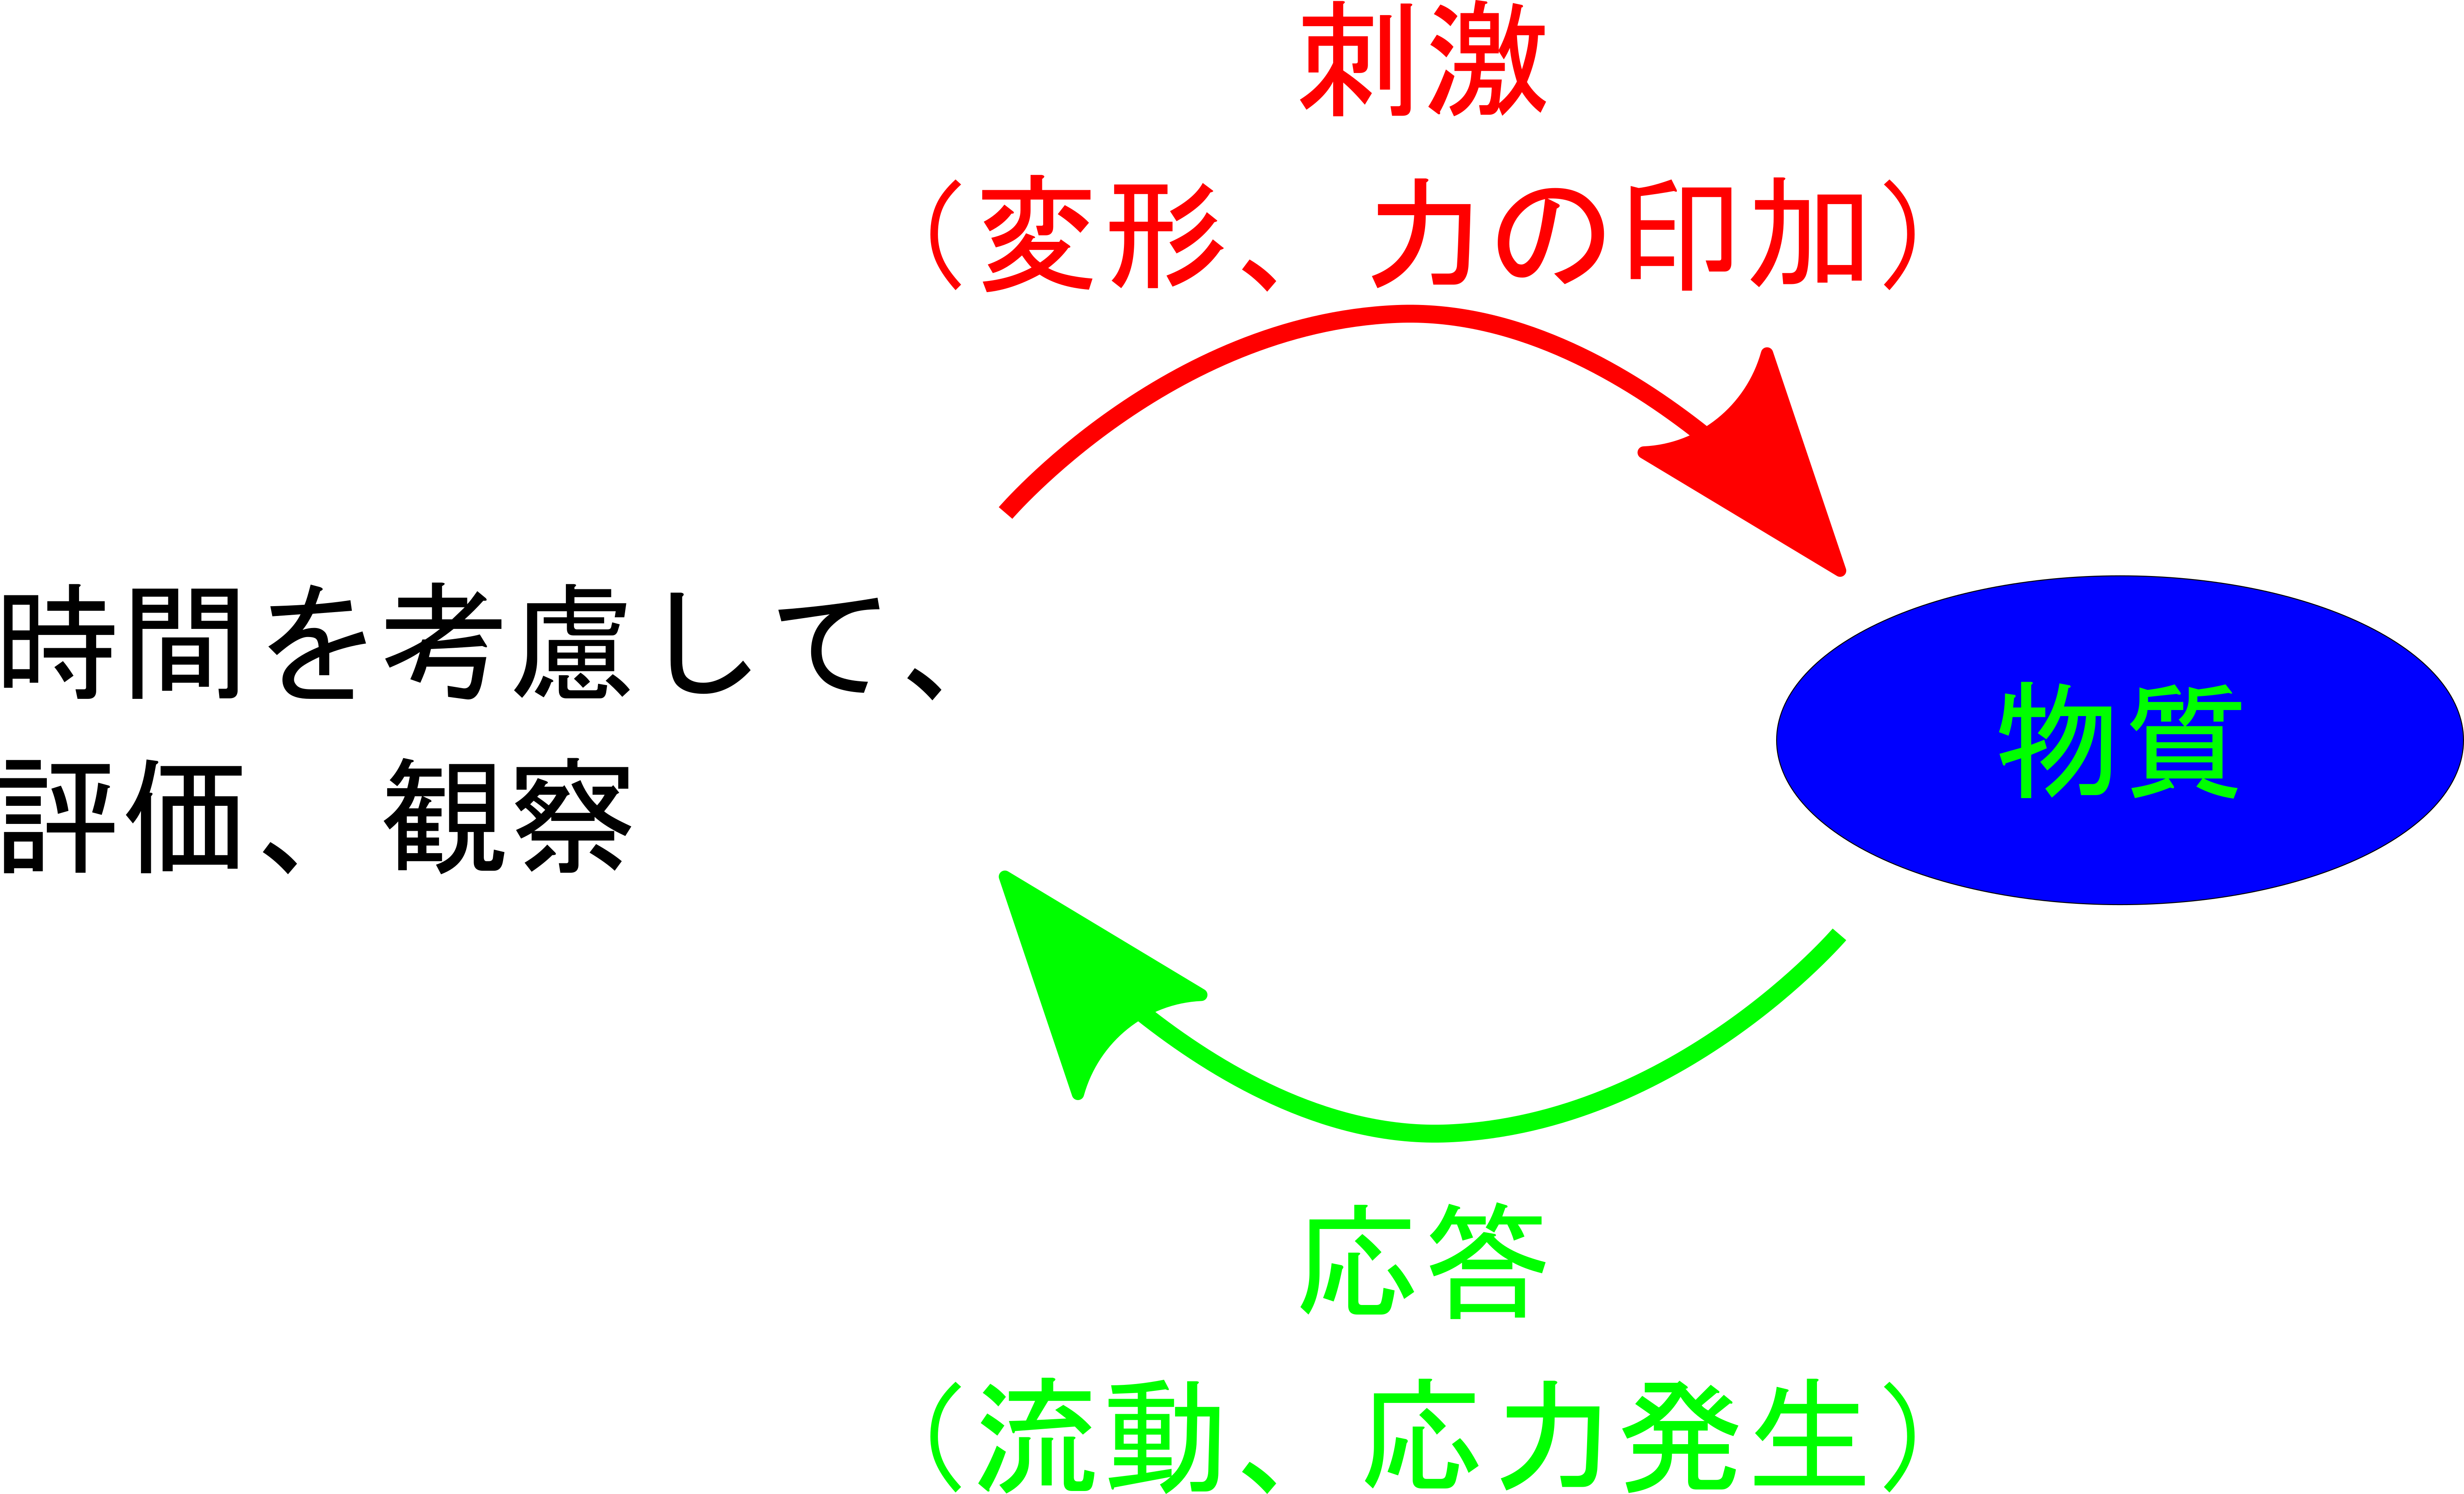
\includegraphics[width=\textwidth]{Rheo_method.png}
		\end{minipage}
		\begin{minipage}{.45\textwidth}
			\large
			\begin{itembox}[l]{レオロジーのやり方}
				\begin{itemize}
					\item 力学的な刺激
					\begin{itemize}
						\item 外力による物質変形
					\end{itemize}
					\item 変形の結果として
					\begin{itemize}
						\item 内部で応力が発生
						\item 流動が生じる場合も
					\end{itemize}
				\end{itemize}
			\end{itembox}
		\end{minipage}
	\caption{レオロジーのやりかた}
	\label{yarikata2}
    \end{center}
\end{figure}

ここでは、わかり易い例として、物質の力学的なレオロジー評価を考えてみましょう。
物質に力学的な刺激を与えるということは、「外力によって物質を変形」させるということに対応します。
このとき、変形の結果として「物質の内部で応力\index{おうりょく@応力}」という応答が生じ、また、流動\index{りゅうどう@流動}が生じる場合もあります。

\subsection{力について}
まず、刺激の源となる「力\index{ちから@力}」というものについての確認から始めていきましょう。

力は以下のように定義されています。
そして、その対象となるものの状態に応じて、「静力学\index{せいりきがく@静力学}」と「動力学\index{どうりきがく@動力学}」の2つに分けて考えることができます。
\large
	\begin{itembox}[l]{力の定義}
		「物体の状態を変化させる原因となる作用で、その作用の大きさを表す物理量」
		\begin{itemize}
			\item 静力学
			\begin{itemize}
				\item 静的状態(時間によって系の位置が変化しない状態)に働く力に関して、
				\item 主として、力の釣り合い\index{ちからのつりあい@力の釣り合い}を議論。
			\end{itemize}
			\item 動力学
			\begin{itemize}
				\item 運動量の変化を伴う質点の移動について議論し、
				\item 相互作用する物体系の運動について議論。
			\end{itemize}
		\end{itemize}
	\end{itembox}
\normalsize

この章でのお話としては、まずは、力の釣り合いを取り扱う静力学としてのアプローチから始めていきます。

\subsection{物質の変形と仕事}

静的な釣り合いとして物質に力\index{ちから@力}を加えることを考えた場合、物質の外から加えた力を「外力\index{がいりょく@外力}」と呼び、そして物質の内部に外力に抵抗する力として「内力\index{ないりょく@内力}」が生じます。
このとき、外力と内力が釣り合うという、「作用・反作用の原理」が成り立ちます。
\large
	\begin{itembox}[l]{静的な釣り合いとしての力}
		\begin{itemize}
			\item 物質の外から加えた力を外力として、
			\item 物質の内部に、外力に抵抗する力として内力が生じ、
			\item 外力と内力が釣り合う。$\Leftrightarrow$ 「作用・反作用の原理」
		\end{itemize}
	\end{itembox}
\normalsize

同時に、外力に対応して、物質は変形します。
この釣り合いのもとでの物質の変形も、仕事となります。
この場合、外力が物質の内部に蓄積された(弾性\index{だんせい@弾性})エネルギーに相当する量の仕事を行ったと考える事ができます\footnote{
	仕事という概念については、次の第 4 章で議論を進めますので、少しお待ち下さい。
}。


\section{弾性体の力学的な刺激と応答}

この節では、わかり易い例として最も単純な固体\index{こたい@固体}のモデルである弾性体\index{だんせいたい@弾性体}を対象として、力学的な刺激と応答ということについて、考えていきます。
なお、弾性体という考え方は、変形を受けてもその起源となる外力を除去すれば、全く元の状態に戻るような性質をあらわしています。
さらに、簡単のために時間の因子も除いて考えることにします。

\subsection{物質のひずみ\index{ひずみ@ひずみ}と応⼒}
ここでは、力学的な刺激として、「外力による物質の変形」を考え、その応答として、「内部での応力発生」を考えます。
% 実際には、変形させるために外力と呼ばれる力を物質に与えるわけですが、そのあたりの細かいことは一旦無視しましょう。

外力\index{がいりょく@外力}を与えた結果として変形が生じたとき、物質はひずみ、内部で応力\index{おうりょく@応力}が発生します。
\large
	\begin{center}
		\begin{minipage}{0.38\textwidth}
			\begin{itembox}[l]{外力による物質の変形}
				\begin{itemize}
					\item 引張変形
					\item せん断変形
				\end{itemize}
			\end{itembox}
		\end{minipage}
		\begin{minipage}{0.38\textwidth}
			\begin{itembox}[l]{変形の結果として}
				\begin{itemize}
					\item 物質はひずむ
					\item 内部で応力が発生
				\end{itemize}
			\end{itembox}
		\end{minipage}
	\end{center}
\normalsize

\subsection{二つの変形とひずみ}
変形を考えていくために、まず、物質を一つの軸に沿って引き伸ばす「引張変形\index{ひっぱりへんけい@引張変形}」とトランプのカードを横にずらしたような「せん断変形\index{せんだんへんけい@せん断変形}」の
二つに、変形を単純化します。

この「せん断変形」のイメージが湧きにくいかもしれません。
たとえば、紙をハサミで切るときにそれぞれの刃が向かい合う方向に移動して紙に力を与えているような状況を想像していただければと思います。
このように互い違いの方向に同じ大きさの力が作用することを、偶力\index{ぐうりょく@偶力}と呼びます。
「せん断変形」は、偶力が働いた結果として生じる変形であると理解してください。

\subsubsection{伸張ひずみ\index{しんちょうひずみ@伸張ひずみ}}
引張変形に対応する物質のひずみ\index{ひずみ@ひずみ}を記述する最も単純なものが、棒状のものを一方向にだけ変形させたときのコーシーひずみ(図 \ref{causy})になります。
このとき、変形量を変形前の長さで除したものがひずみ\index{ひずみ@ひずみ} (一般に、コーシーひずみのような伸張ひずみはギリシア文字の $\varepsilon$ と表記) となります。
\begin{figure}[htb]
	\begin{center}
		\begin{minipage}{0.45\textwidth}
			\large
			\begin{itembox}[l]{コーシーひずみ:}
				\vspace{-3mm}
				\begin{align*}
					\varepsilon_c &= \dfrac{\text{\textbf{変形量}}}{\text{\textbf{変形前の長さ}}} \\
					&=\dfrac{\Delta L}{L_0} = \dfrac{L-L_0}{L_0}
				\end{align*}
			\end{itembox}
		\end{minipage}
		\begin{minipage}{0.45\textwidth}
			\begin{center}
				\includegraphics[width=0.9\textwidth]{Causy.png}
			\end{center}
		\end{minipage}
		\caption{コーシーひずみ}
		\label{causy}
	\end{center}
\end{figure}

\subsubsection{せん断ひずみ\index{せんだんひずみ@せん断ひずみ}}
また、せん断変形\index{せんだんへんけい@せん断変形}によるひずみ (せん断ひずみはギリシア文字の $\gamma$ と表記) は、図 \ref{shear} に示したように、変形方向への変形量をサンプルの厚みで除した形で表すことになります。
このとき、高さ $h$ を一定とし、変形前後での体積変化もないものと考えています。
\begin{figure}[htb]
	\begin{center}
		\begin{minipage}{0.45\textwidth}
			\large
			\begin{itembox}[l]{せん断ひずみ:}
				\vspace{-3mm}
				\begin{align*}
					\gamma &= \dfrac{\text{\textbf{変形方向への変形量}}}{\text{\textbf{サンプルの厚み}}} \\
					&=\dfrac{x}{h}
				\end{align*}
			\end{itembox}
		\end{minipage}
		\begin{minipage}{0.45\textwidth}
			\begin{center}
				\includegraphics[width=0.9\textwidth]{Shear.png}
			\end{center}
		\end{minipage}
		\caption{せん断ひずみ}
		\label{shear}
	\end{center}
\end{figure}

なお、ひずみ\index{ひずみ@ひずみ}は、長さを長さで割ったものとなりますので、次元を持たない無次元量であることに注意してください。

\subsection{応力のイメージ}
応力\index{おうりょく@応力}とは、物質の内部に生じている力の大きさを表す物理量であり、その表す意味は単位面積あたりに働く内部の力ということになります。
したがって、その次元は以下のように書けます。
\large
	\begin{itembox}[l]{応力の次元}
		\vspace{-3mm}
		\begin{align*}
			[\text{応力}] = \dfrac{[\text{力}]}{[\text{面積}]} = \dfrac{[\mathrm{N}]}{[\mathrm{m}]^2} = [\mathrm{Pa}]
		\end{align*}
	\end{itembox}
\normalsize

棒状の物質に引っ張り変形を与えた場合の、外力と応力\index{おうりょく@応力}のイメージを図 \ref{stress} に示しました。
このとき、棒の長手方向にはどの位置で切断したとしても、同一の応力\index{おうりょく@応力}が働いていることに注意してください。
\begin{figure}[htb]
	\begin{center}
		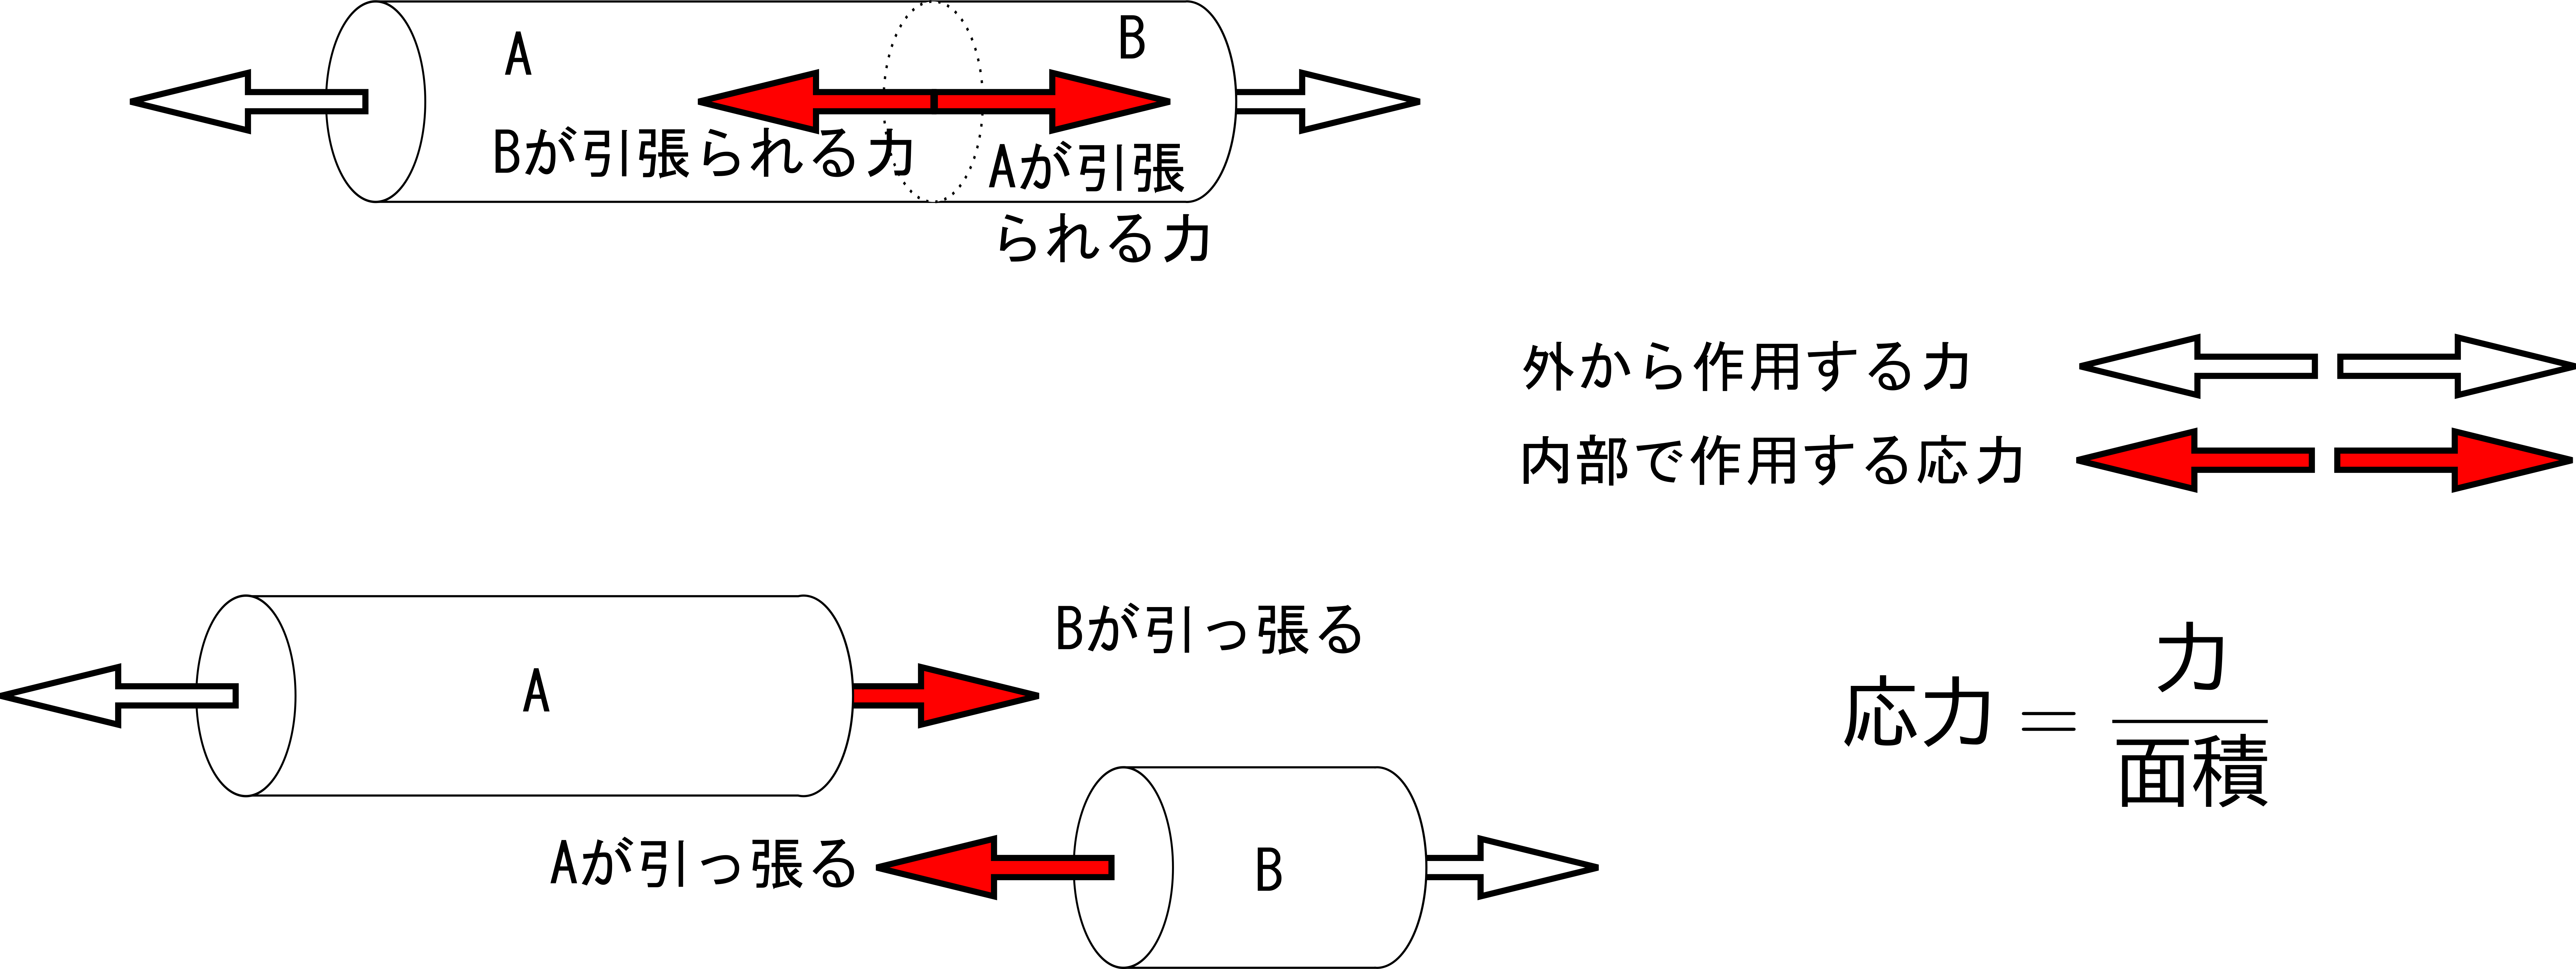
\includegraphics[width=.9\textwidth]{Stress.png}
		\caption{応力のイメージ}
		\label{stress}
	\end{center}
\end{figure}

\subsubsection{伸長応力\index{しんちょうおうりょく@伸長応力} $\sigma$}
伸長時に働く応力は、一般に、ギリシア文字の $\sigma$ と表記します。
表式とすれば、以下のように書くことができます。
\begin{align*}
	\sigma = \dfrac{F}{A}
\end{align*}
なお、$F$ は外部から加えた外力を、$A$ は内部で応力\index{おうりょく@応力}が働く断面積ということになります。

繰り返しますが、応力\index{おうりょく@応力}は単位面積あたりに働く内部の力ですから、図 \ref{elong_stress} に示したように細い棒と入れ替えて断面積が小さくなれば、それに反比例して応力\index{おうりょく@応力}は増加します。
\begin{figure}[htb]
	\begin{center}
		\begin{minipage}{0.45\textwidth}
			\large
			\begin{align*}
				\sigma &= \dfrac{\text{\textbf{与えた力}}}{\text{\textbf{断面積}}} \\
					&=\dfrac{F}{A}
			\end{align*}
			\begin{itemize}
				\item $F$ は外部から加えた外力
				\item $A$ は内部で応力\index{おうりょく@応力}が働く断面積
			\end{itemize}
			\begin{itembox}[l]{同一の外力でも}
				\begin{itemize}
					\item 断面積が小さくなれば、
					\item 反比例して応力\index{おうりょく@応力}は増加
				\end{itemize}
			\end{itembox}
		\end{minipage}
		\begin{minipage}{0.45\textwidth}
			\begin{center}
				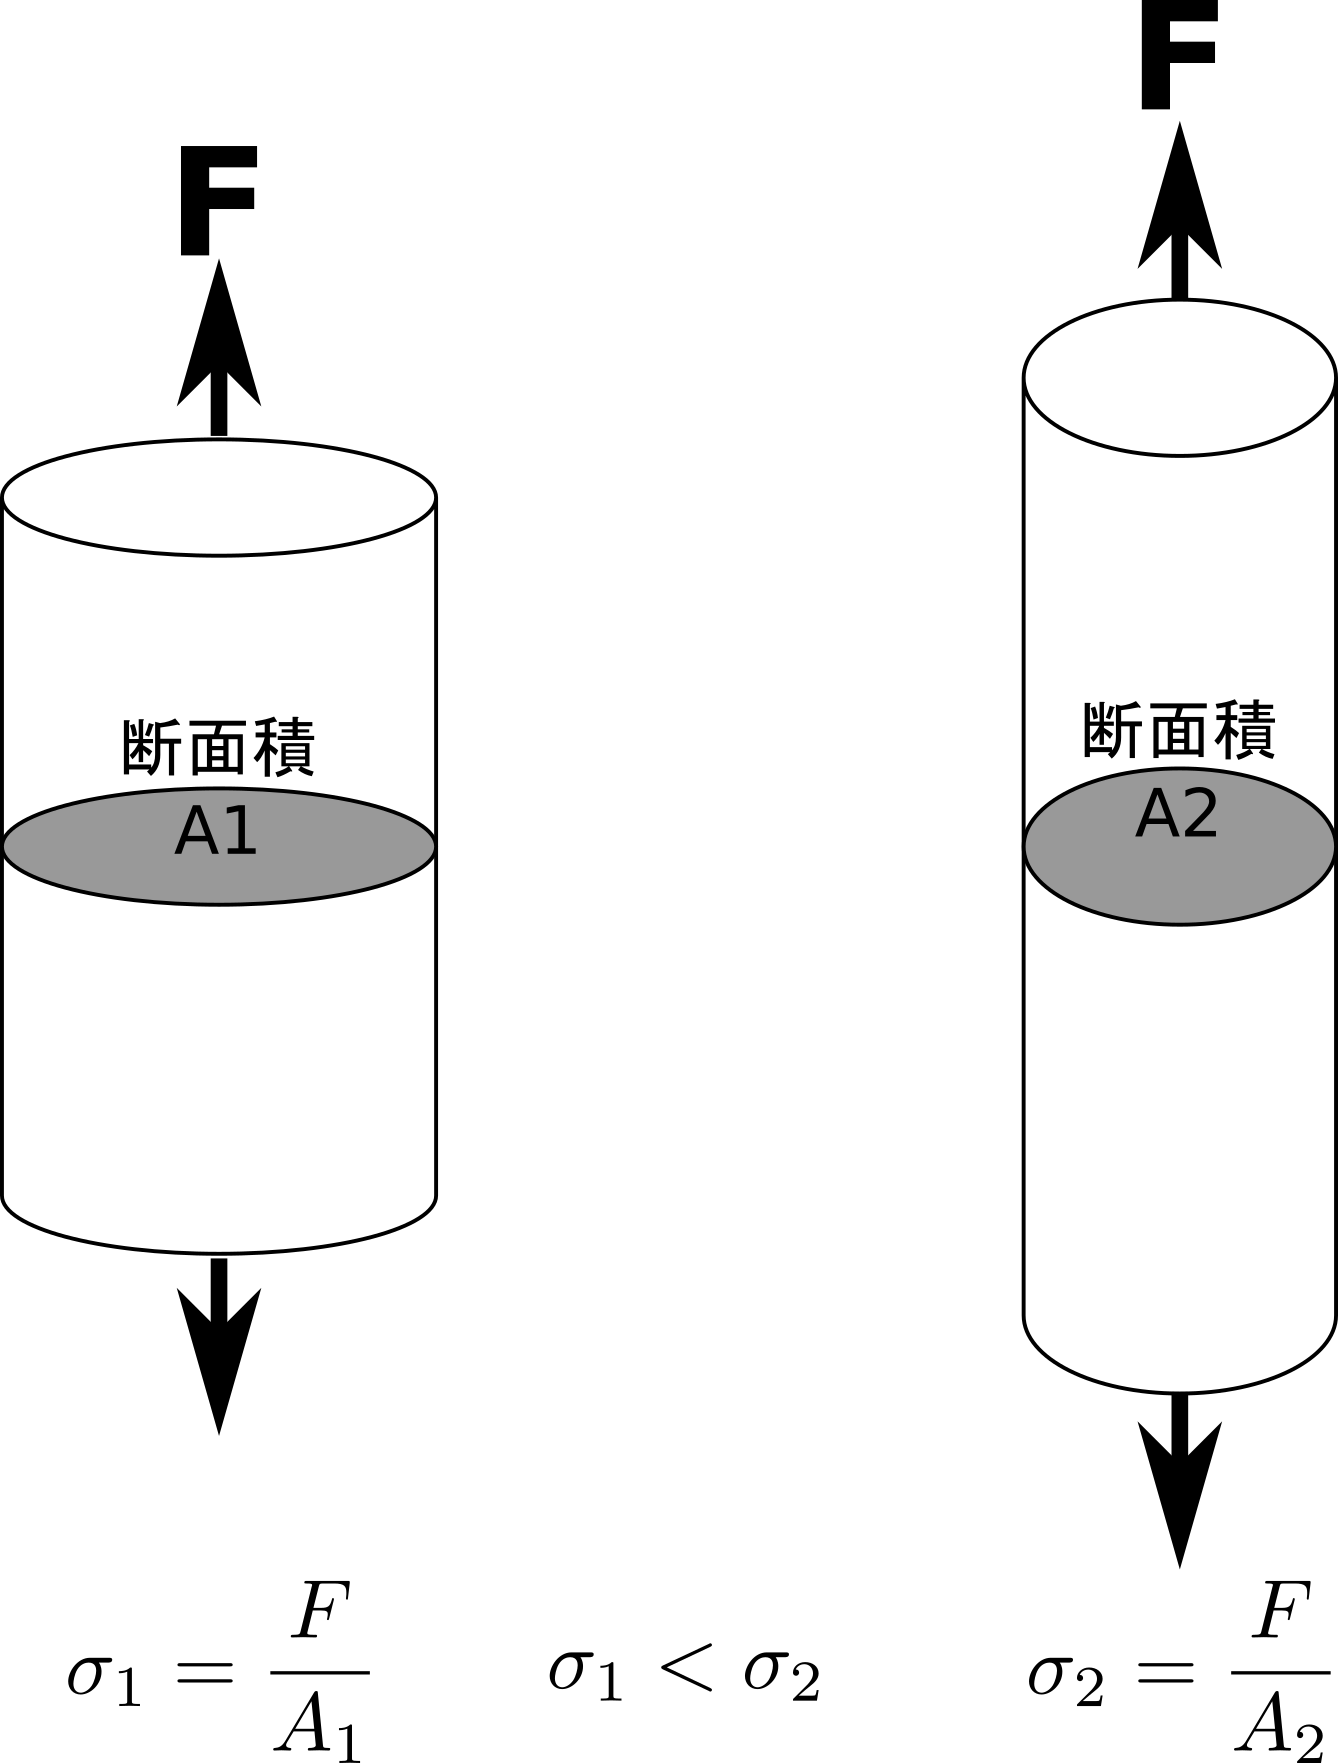
\includegraphics[width=.8\textwidth]{elong_stress.png}
			\end{center}
		\end{minipage}
		\caption{伸長応力}
		\label{elong_stress}
	\end{center}
\end{figure}

\subsubsection{せん断応力 $\tau$}
互いに向かい合う同じ大きさの力である偶力 $F$ を作用させてせん断変形\index{せんだんへんけい@せん断変形}を生じた場合のせん断応力\index{せんだんおうりょく@せん断応力}(せん断の場合は、応力を $\tau$ と表記)のイメージを、図 \ref{shear_stress} に示しました。
なお、力を働かせた上面の面積が $A$ であることに注意してください。
\begin{figure}[htb]
	\begin{center}
		\begin{minipage}{0.45\textwidth}
			\large
			\begin{itembox}[l]{せん断応力 $\tau$}
				\vspace{-3mm}
				\begin{align*}
					\tau &= \dfrac{\text{\textbf{与えた力}}}{\text{\textbf{働かせた面積}}} \\
					&= \dfrac{F}{A}
				\end{align*}
			\end{itembox}
		\end{minipage}
		\begin{minipage}{0.45\textwidth}
			\begin{center}
			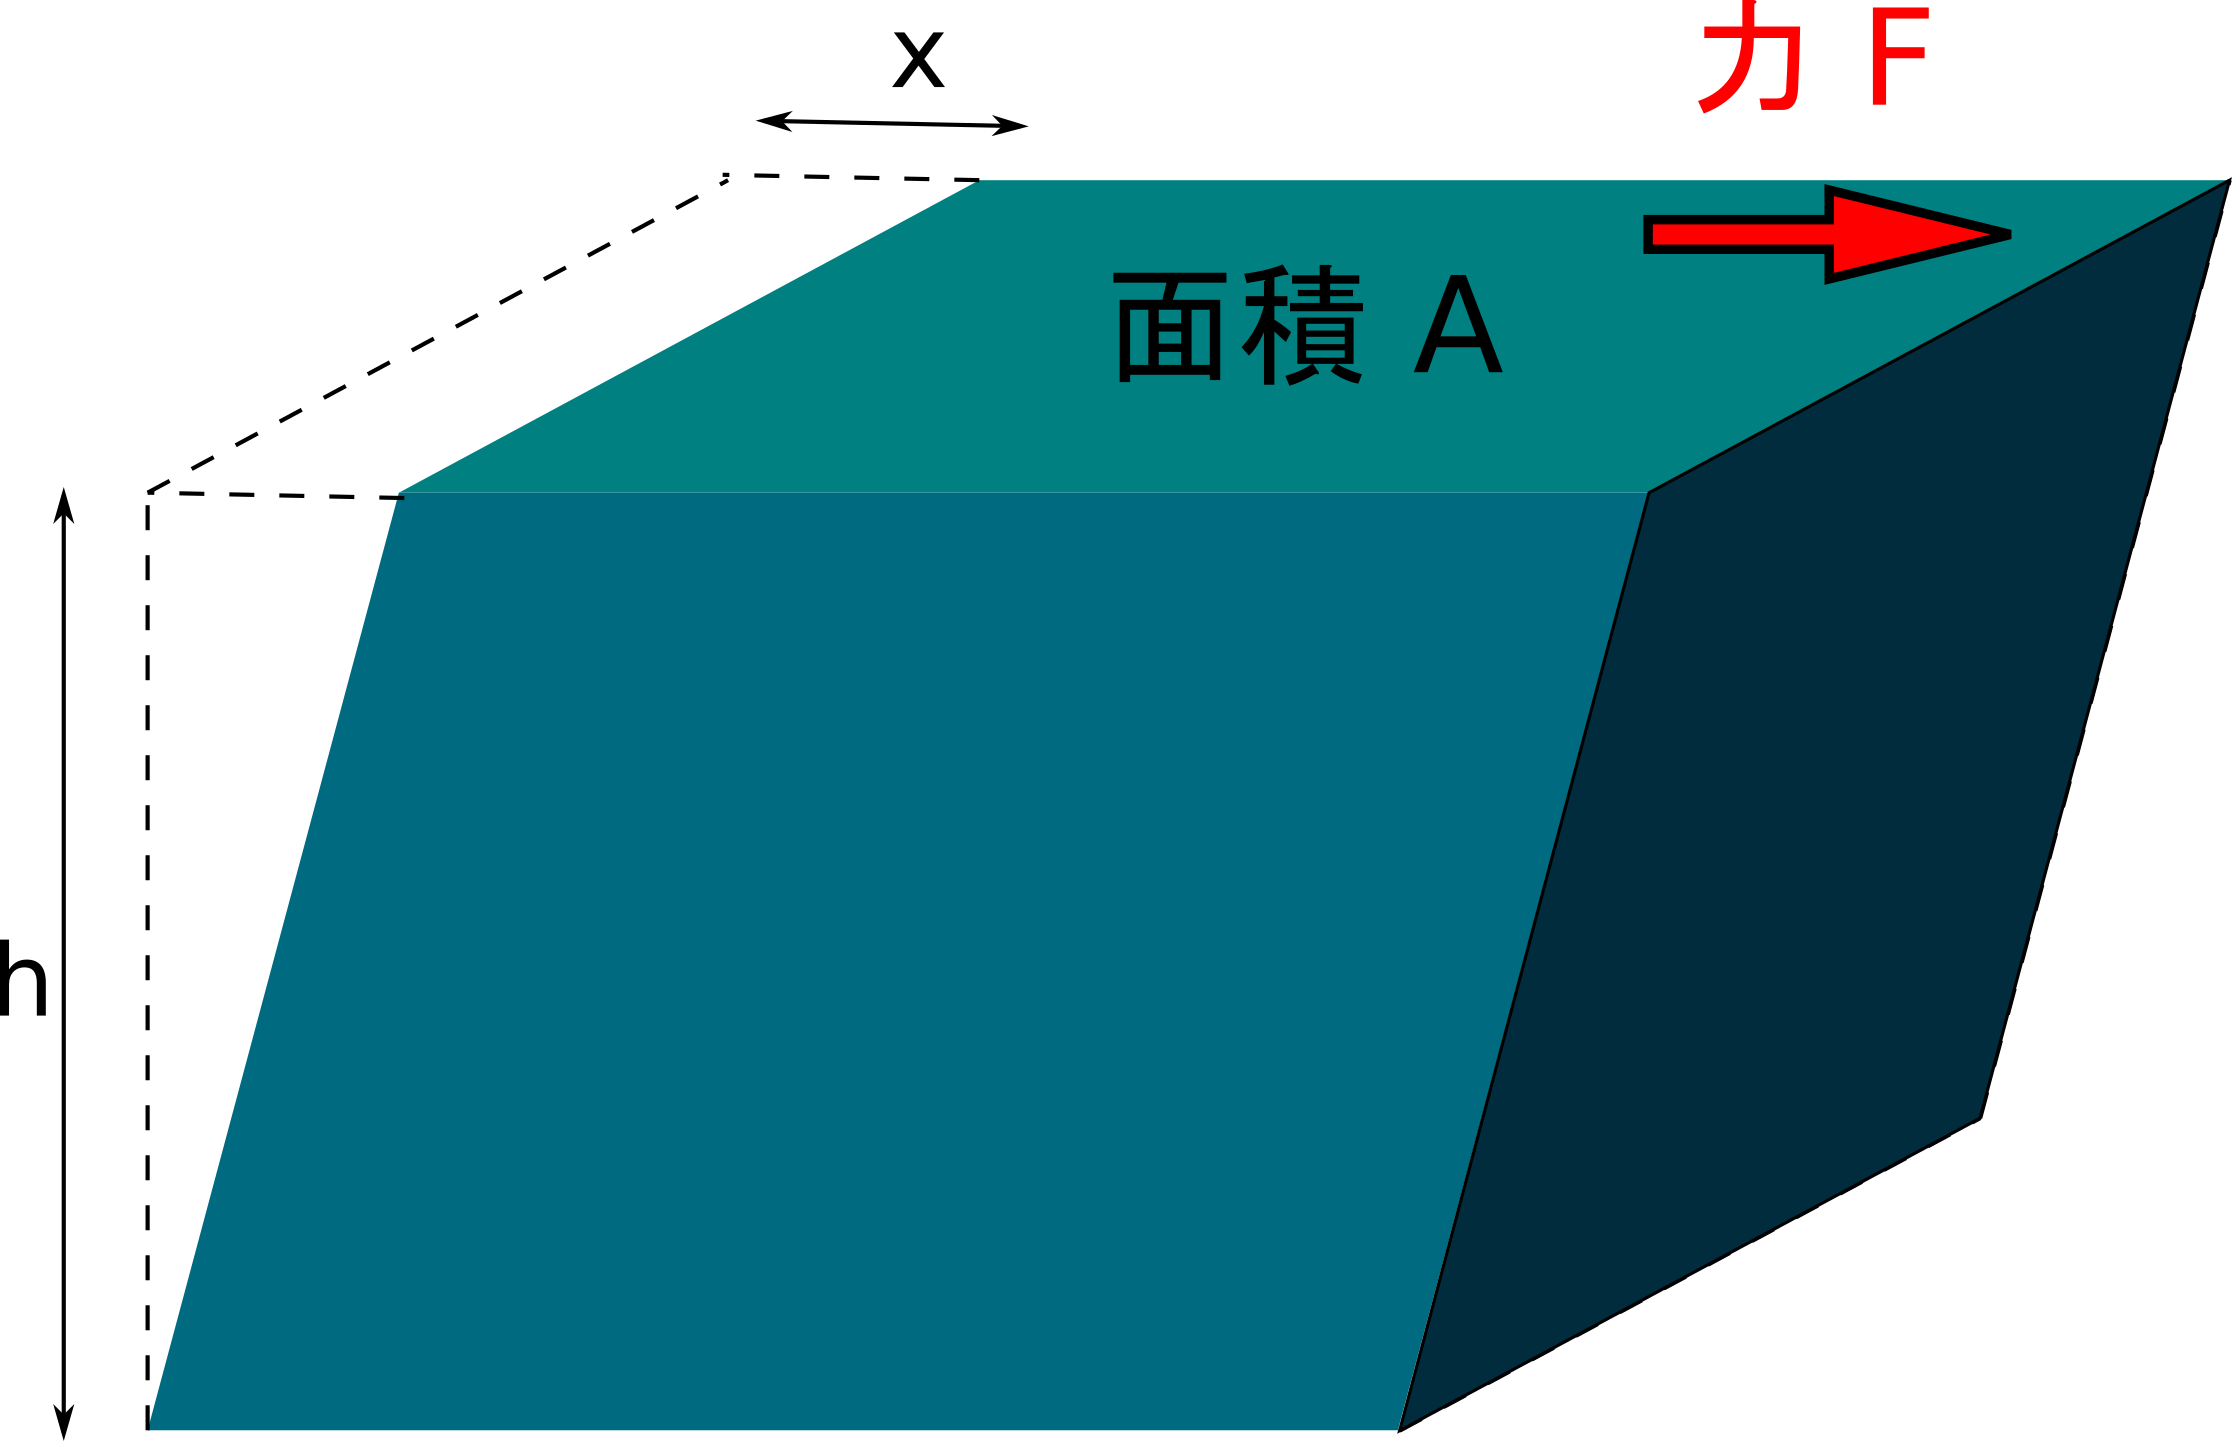
\includegraphics[width=.9\textwidth]{shear_2.png}
			\end{center}
		\end{minipage}
		\caption{せん断応力}
		\label{shear_stress}
	\end{center}
\end{figure}

このとき、サンプルの厚さ方向には、どの位置であっても同一のせん断応力\index{せんだんおうりょく@せん断応力}が作用していることになり、伸張ひずみの場合と同様に厚さ方向にはどの位置で切断したとしても同一の偶力が作用していることになります。

このせん断応力のイメージは、トランプのカードが重なったデッキを想像することで、理解しやすくなるかもしれません。
つまり、デッキの間に挟まったカードは、一枚上のカードと下のカードによって偶力を受けることになるわけです。
\begin{figure}[htbp]
	\begin{center}
		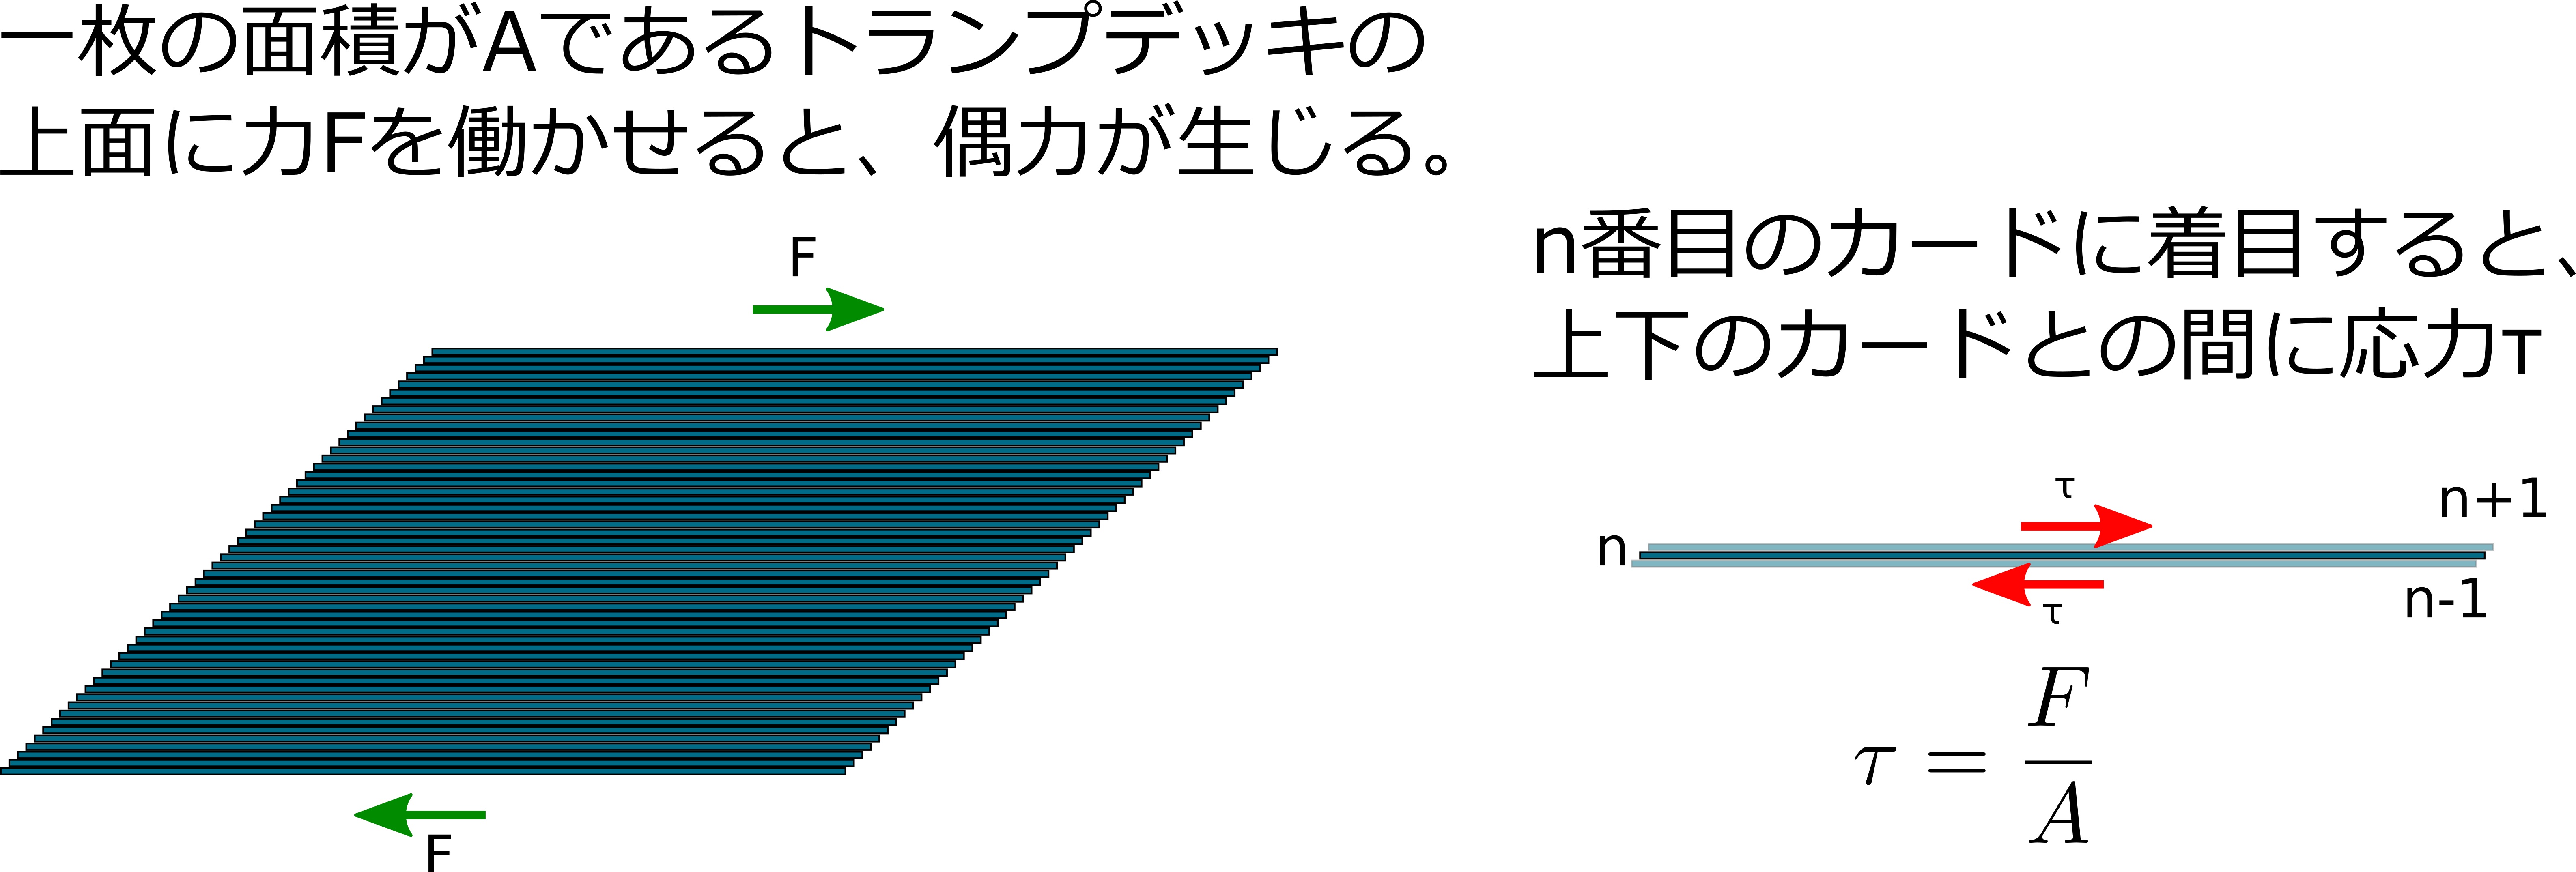
\includegraphics[width=.9\textwidth]{trump_deck.png}
		\caption{内部でのイメージ}
		\label{trump}
	\end{center}
\end{figure}

\section{力学モデルについて}
\subsection{弾性体のモデル}

ここまで刺激と応答の例として使ってきた弾性体を、物質として評価する方法について考えてみましょう。
つまり、弾性体の力学応答を書き表すことが出来るモデルを数式として表すことで、異なる物質を定量的に比較できるようになることを目指すわけです。

\subsubsection{Hooke の法則}

これまでの経験から、弾性体はあたかもバネのように取り扱うことができることが知られています。
そして、バネの力学的な振る舞いには、イギリスの物理学者 Robert Hooke が見出した「Hooke の法則」\index{ふっくのほうそく@Hooke の法則}と呼ばれる以下の関係があることがわかっています。
\begin{figure}[htb]
	\begin{center}
		\begin{minipage}{0.45\textwidth}
			\large
			\begin{itembox}[l]{Hooke の法則}
				\vspace{-3mm}
				\begin{align*}
					\text{外力} &= \text{比例定数} \times \text{変位量} \\[8pt]
					F(x) &= k x
				\end{align*}
			\end{itembox}
		\end{minipage}
		\begin{minipage}{0.45\textwidth}
			\begin{center}
			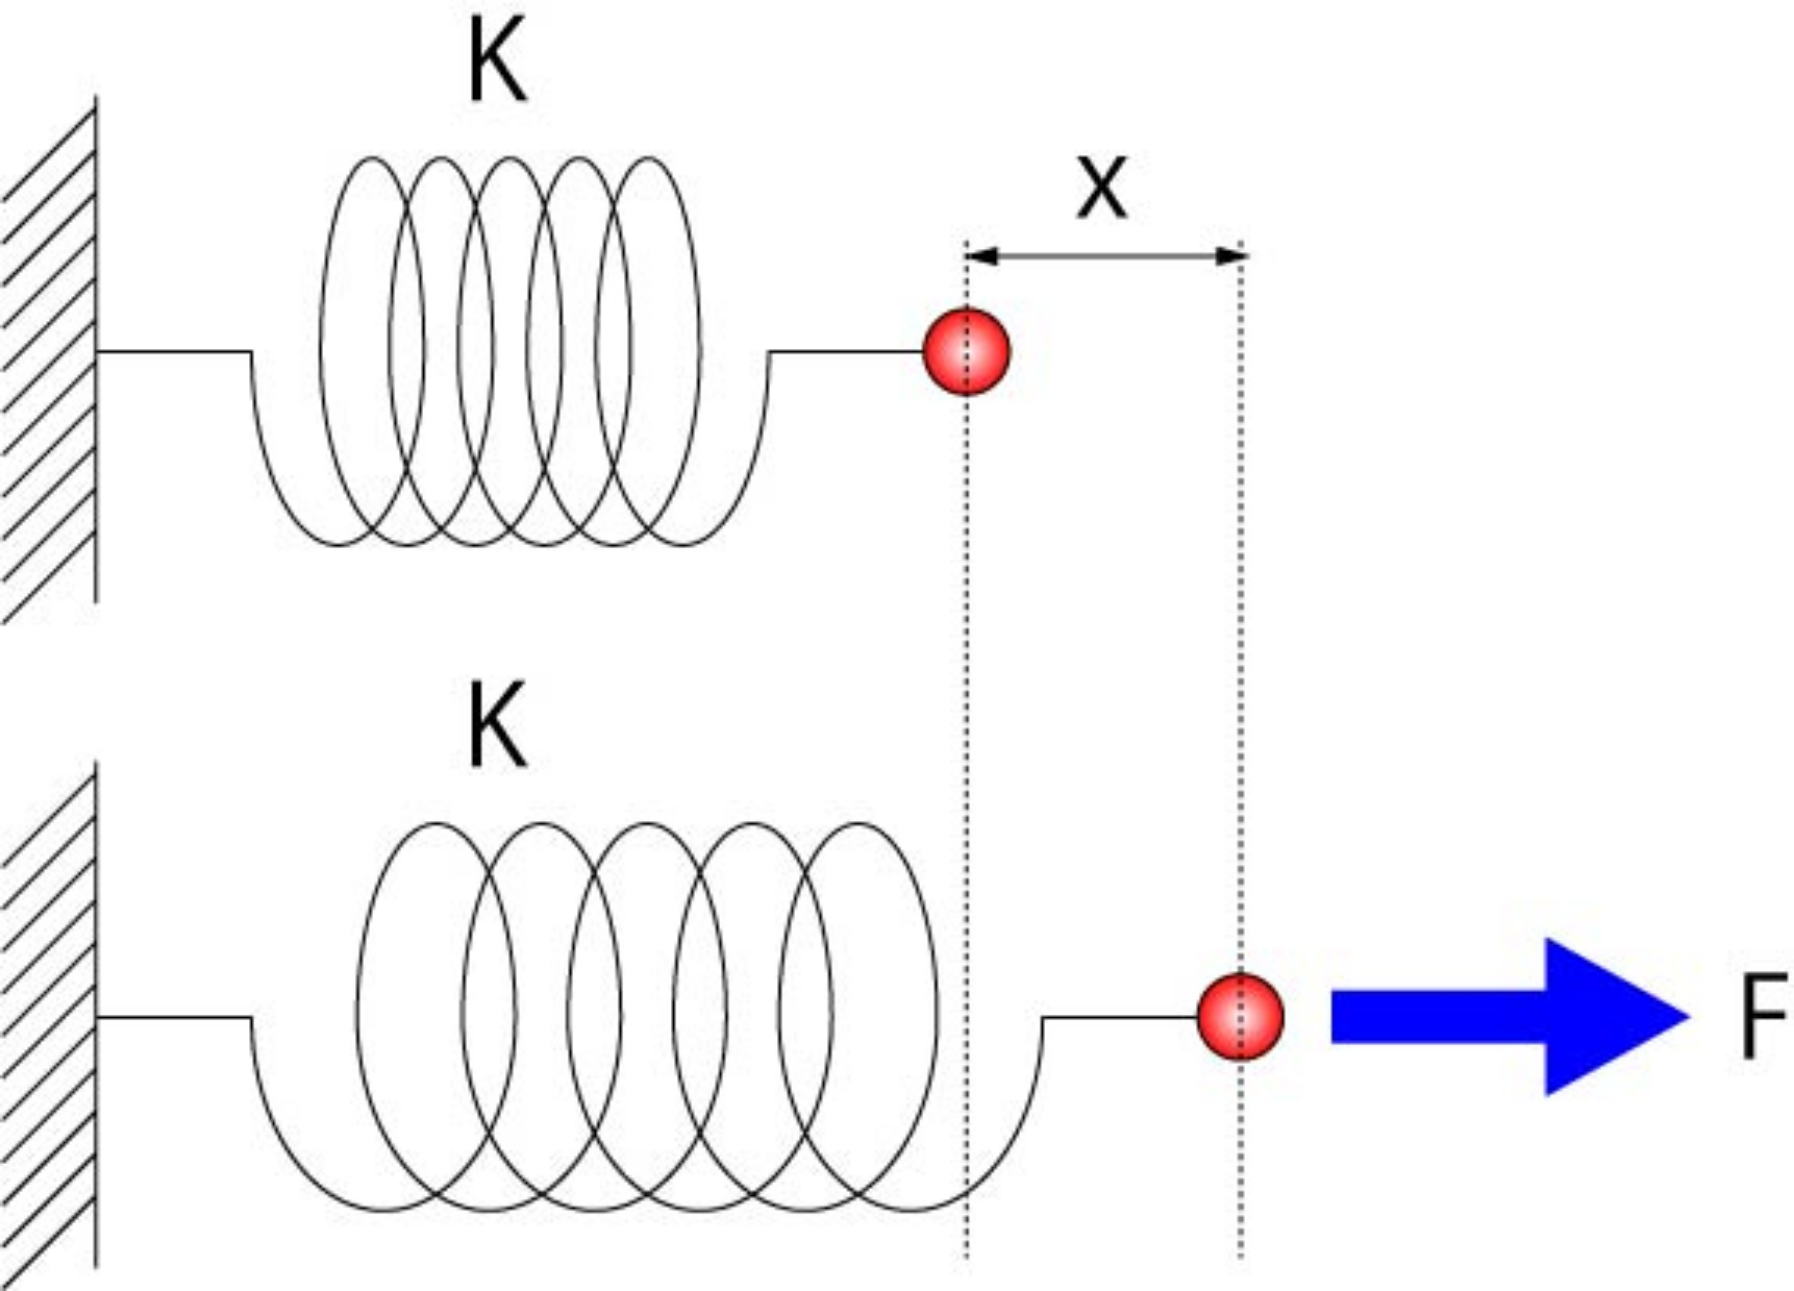
\includegraphics[width=.8\textwidth]{spring.png}
			\end{center}
		\end{minipage}
		\caption{Hooke の法則}
		\label{hook}
	\end{center}
\end{figure}

この式は、外力 $F$ と変位量 $x$ が比例(比例定数が $k$)することを表しています。

\subsubsection{弾性体の力学モデル}

弾性体の力学モデルは、上述のHooke の法則に従う形で、以下のようになります。
\begin{figure}[htb]
	\begin{center}
		\begin{minipage}{0.45\textwidth}
			\large
			\begin{itembox}[l]{弾性体の伸張変形}
				\begin{itemize}
					\item 変形ひずみ $\varepsilon$ と比例して、
					\item 応力 $\sigma$ が生じ、
					\item 比例定数が引張弾性率\index{ひっぱりだんせいりつ@引張弾性率} $E$
				\end{itemize}
			\end{itembox}
		\end{minipage}
		\begin{minipage}{0.45\textwidth}
			\begin{center}
			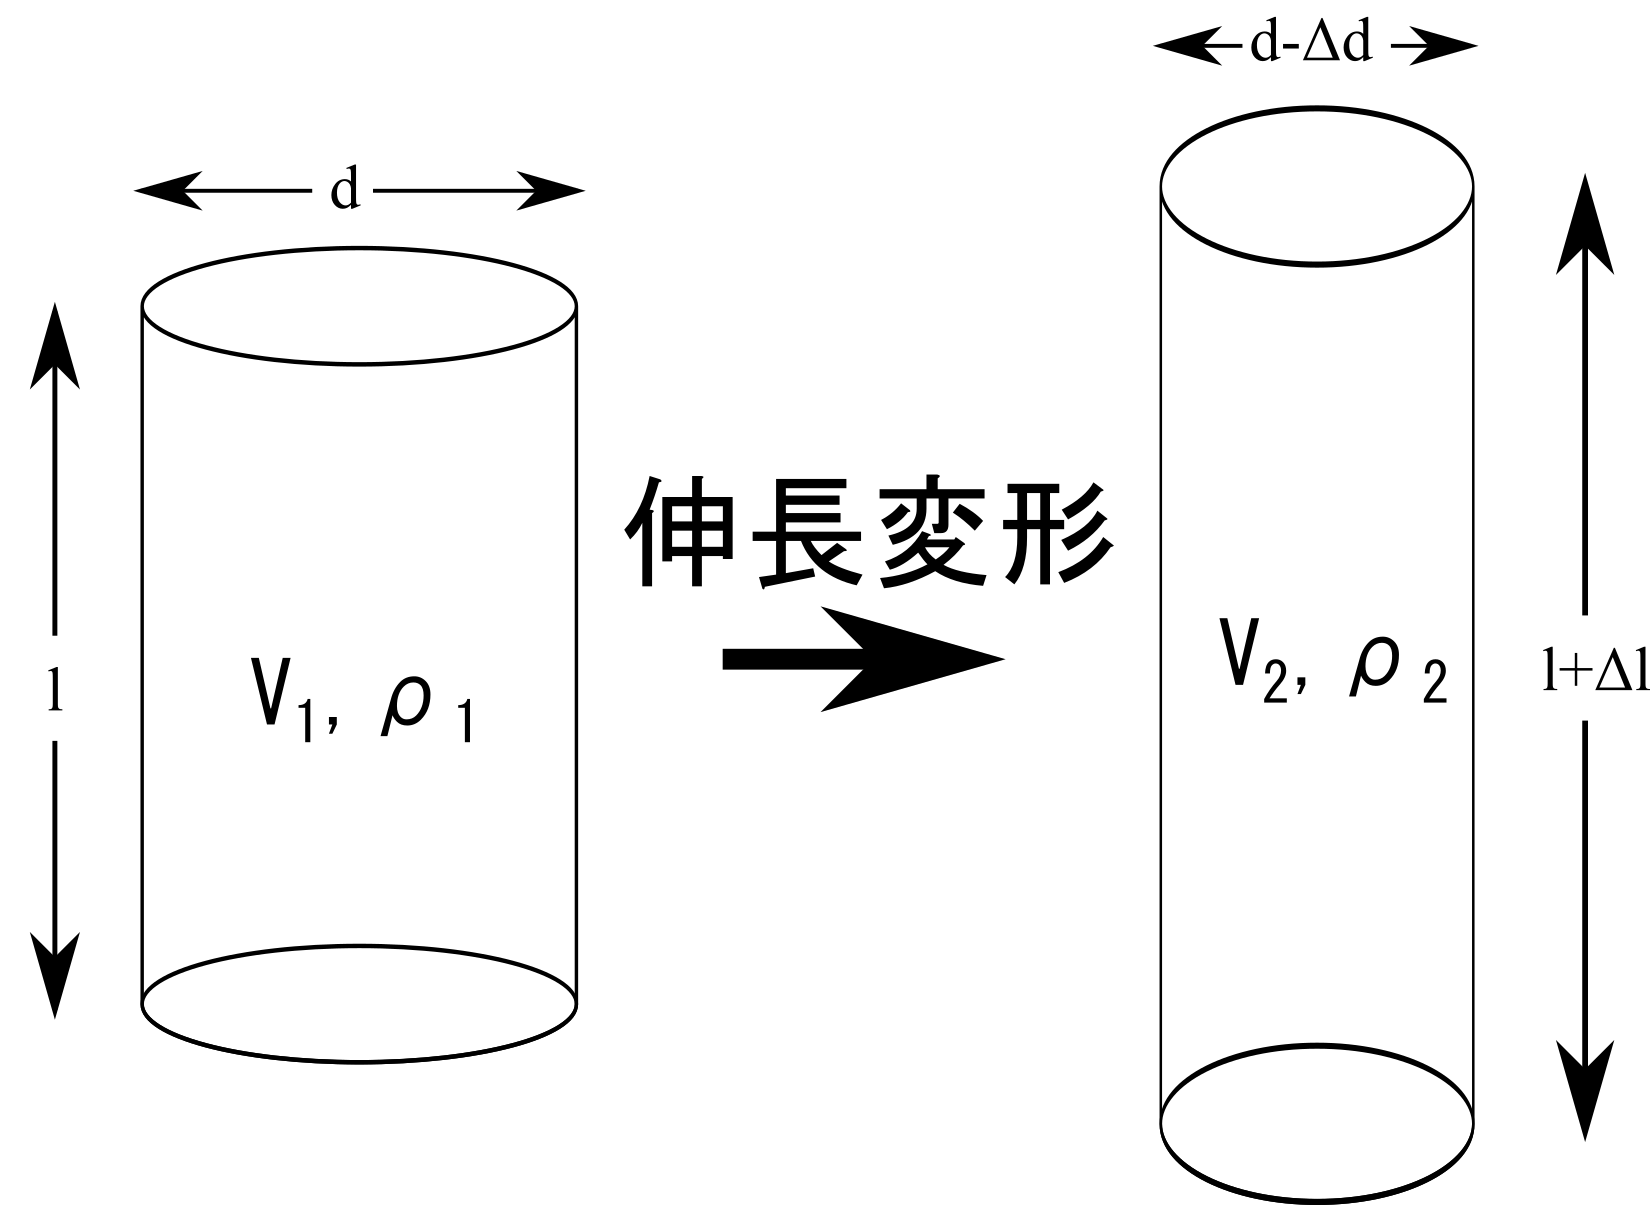
\includegraphics[width=.8\textwidth]{hook_law.png}
			\end{center}
		\end{minipage}
		\caption{弾性体の伸張変形モデル}
		\label{eq:hookian}
	\end{center}
\end{figure}

この関係を表式とすれば、下式となります。
\begin{align}
	\text{伸長応力} &= \text{引張弾性率\index{ひっぱりだんせいりつ@引張弾性率}} \times \text{ヘンキーひずみ} \notag \\
	\sigma &= E \varepsilon 
	\label{eq:hookian2}
\end{align}
なお、ひずみ\index{ひずみ@ひずみ}は無次元量でしたから、引張弾性率\index{ひっぱりだんせいりつ@引張弾性率} $E$ は伸長応力 $\sigma$ と同じ次元である [Pa] となります。

ここで、気をつけていただきたいのは、弾性体の Hooke モデルでは全体のひずみ\index{ひずみ@ひずみ}に比例するのは応力\index{おうりょく@応力}であるということです。
何度も繰り返しましたように、応力\index{おうりょく@応力}とは、働いている力を面積で除したものです。
したがって、伸張に伴って変化した面積に対応した応力を考える必要があります。

また、この Hooke モデルは、せん断変形の場合にも使うことができます。
このときは、以下に示したように、
\begin{align}
	\text{せん断応力} &= \text{せん断弾性率\index{せんだんだんせいりつ@せん断弾性率}} \times \text{せん断ひずみ} \notag \\
	\tau &= G \gamma
\end{align}
せん断変形の場合は、比例定数はせん断弾性率\index{せんだんだんせいりつ@せん断弾性率}と呼ばれ、$G$ で表され、せん断応力\index{せんだん@せん断応力} $\tau$ と同じ次元である [Pa] となります。

\subsection{液体の変形と応答}

ここまでの議論は、固体\index{こたい@固体}のモデルとして弾性体を変形の対象として行ってきました。
次に、液体\index{えきたい@液体}のモデルを考えてみましょう。

\subsubsection{流れるという性質}
液体\index{えきたい@液体}と固体\index{こたい@固体}の違いについては後ほど詳しく議論しますが、ここでは非常に単純に外力によって変形されたら元には戻れない「流れる」という性質を持った物質と考えてください。
この性質を簡単にまとめると以下のようになります。
\begin{figure}[htb]
	\begin{center}
		\begin{minipage}{0.55\textwidth}
			\large
			\begin{itembox}[l]{流れるという性質}
				\begin{itemize}
					\item コップの中ではじっとしている。
					\item 変形を与えると流れる
					\begin{itemize}
						\item 元には戻らない。
						\item 変形を止めれば、応力も消失
					\end{itemize}
					\item 応答を見るのが困難
					\begin{itemize}
						\item 変形を続けながら応力を測る
						\item 液体内部の変形と応力を見積る
					\end{itemize}
				\end{itemize}
			\end{itembox}
		\end{minipage}
		\begin{minipage}{0.35\textwidth}
			\begin{center}
			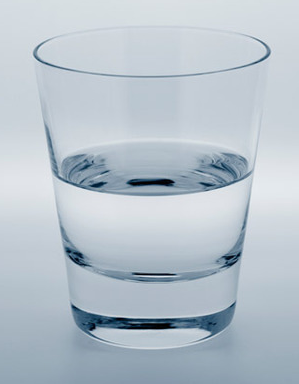
\includegraphics[width=.6\textwidth]{cup_water.png}
			\end{center}
		\end{minipage}
		\caption{流れるという性質}
		\label{fig:flow}
	\end{center}
\end{figure}

この「流れる」という性質のために、流体\index{りゅうたい@流体}の応答を測ろうとする場合には、固体\index{こたい@固体}と考え方を変える必要があります。
したがって、液体\index{えきたい@液体}の評価は主としてその形状を維持しやすい「せん断変形\index{せんだんへんけい@せん断変形}」により行われる場合が多くなります。
そして、測定の間、せん断変形を与え続ける必要があります。

\subsubsection{液体の性質を直感的に理解}

液体\index{えきたい@液体}が生じる力を直感的に理解するために、プールでの水中歩行を考えてみましょう。

腰以上に水に浸かって、ゆっくりと移動しているときには、水から受ける抵抗はそれほど大きいものではありません。
ところが、速く歩こうとすると、とたんに水の抵抗は大きくなってしまいます。

\begin{figure}[htb]
	\begin{center}
		\begin{minipage}{0.55\textwidth}
			\large
			\begin{itembox}[l]{液体の性質}
				変形させる速度が変わると、\\生じる力も変わる。
				\begin{itemize}
					\item ゆっくりと歩いて移動(上の図)
					\begin{itemize}
						\item 受ける抵抗はそれほど大きくない。
					\end{itemize}
					\item 走って速く移動(下の図)
					\begin{itemize}
						\item 速く歩こうとすると、とたんに\\水の抵抗は大きくなります。
					\end{itemize}
				\end{itemize}
			\end{itembox}
		\end{minipage}
		\begin{minipage}{0.35\textwidth}
			\begin{center}
			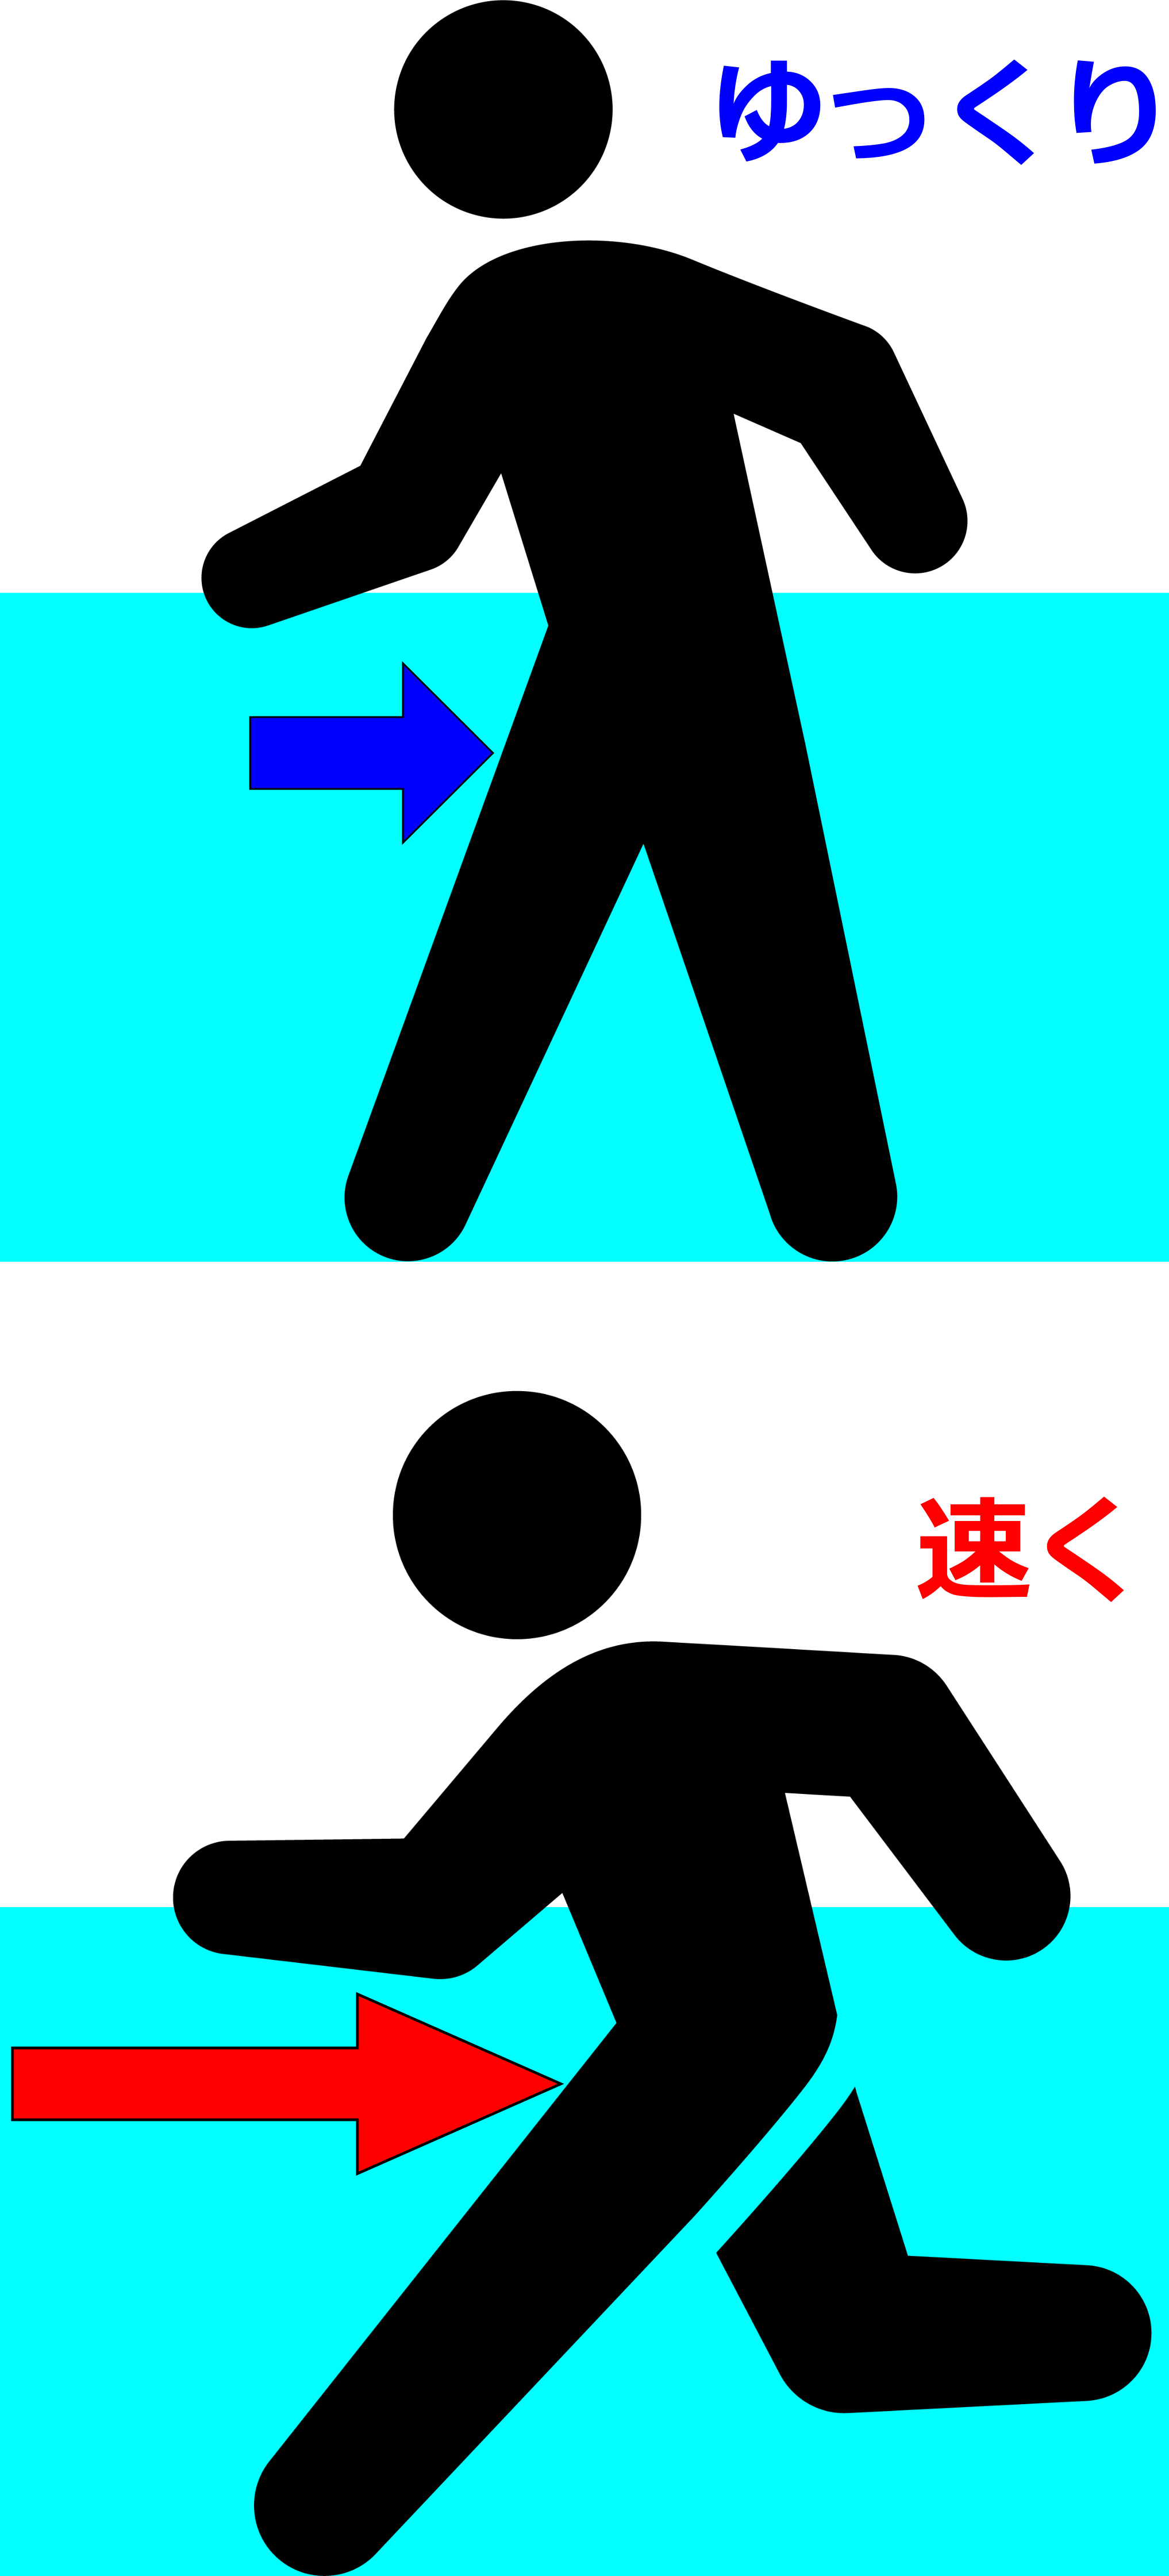
\includegraphics[width=.5\textwidth]{pool_walking.png}
			\end{center}
		\end{minipage}
		\caption{プールでの水中歩行}
		\label{pool_walk}
	\end{center}
\end{figure}

このことから、液体\index{えきたい@液体}の性質として、変形させる速度が変わると生じる力も変わって、速い変形に対しては応力も大きくなることがわかります。


\subsection{液体\index{えきたい@液体}の力学モデル}

\subsubsection{ ニュートンの法則}
では、液体\index{えきたい@液体}の力学的な応答を記述するモデルはどうなるのでしょうか。
これは、古典力学の土台を築いた Sir Isaac Newton が、流れのせん断応力\index{せんだん@せん断応力} $\tau$ とせん断速度\index{せんだん@せん断速度} $\dot{\gamma}$ (速度勾配\index{そくどこうばい@速度勾配})との間に比例関係を見出しています。

実際の実験は、図 \ref{nijyu} に示したような二重になった円筒中に試料となる液体\index{えきたい@液体}を入れ、内部の円筒を回転させながらそのときに生じる力を測定します。
内部に入った円筒の回転速度を変化させることでせん断速度\index{せんだん@せん断速度}を変化させ、そのときに生じるせん断応力との間に比例関係があることを見出しました。

この比例関係を式で表せば、
	\begin{align}
		\text{せん断応力} &= \text{比例定数} \times \text{せん断速度} \notag \\
		\tau &= \eta \dot{\gamma}
	\end{align}
式中で示した比例定数が、物質の流れ易さを表す指標である「粘度\index{ねんど@粘度}」となります。
\begin{figure}[htb]
	\begin{center}
		\begin{minipage}{0.6\textwidth}
			\large
			\begin{itembox}[l]{ニュートンの法則}
				\vspace{-3mm}
				\begin{align*}
					\text{せん断応力} &= \text{比例定数} \times \text{せん断速度} \notag \\
					\tau &= \eta \dot{\gamma}
				\end{align*}
				比例定数 $\eta$ が、物質の流れ易さを表す「粘度\index{ねんど@粘度}」
			\end{itembox}
		\end{minipage}
		\begin{minipage}{0.3\textwidth}
			\begin{center}
			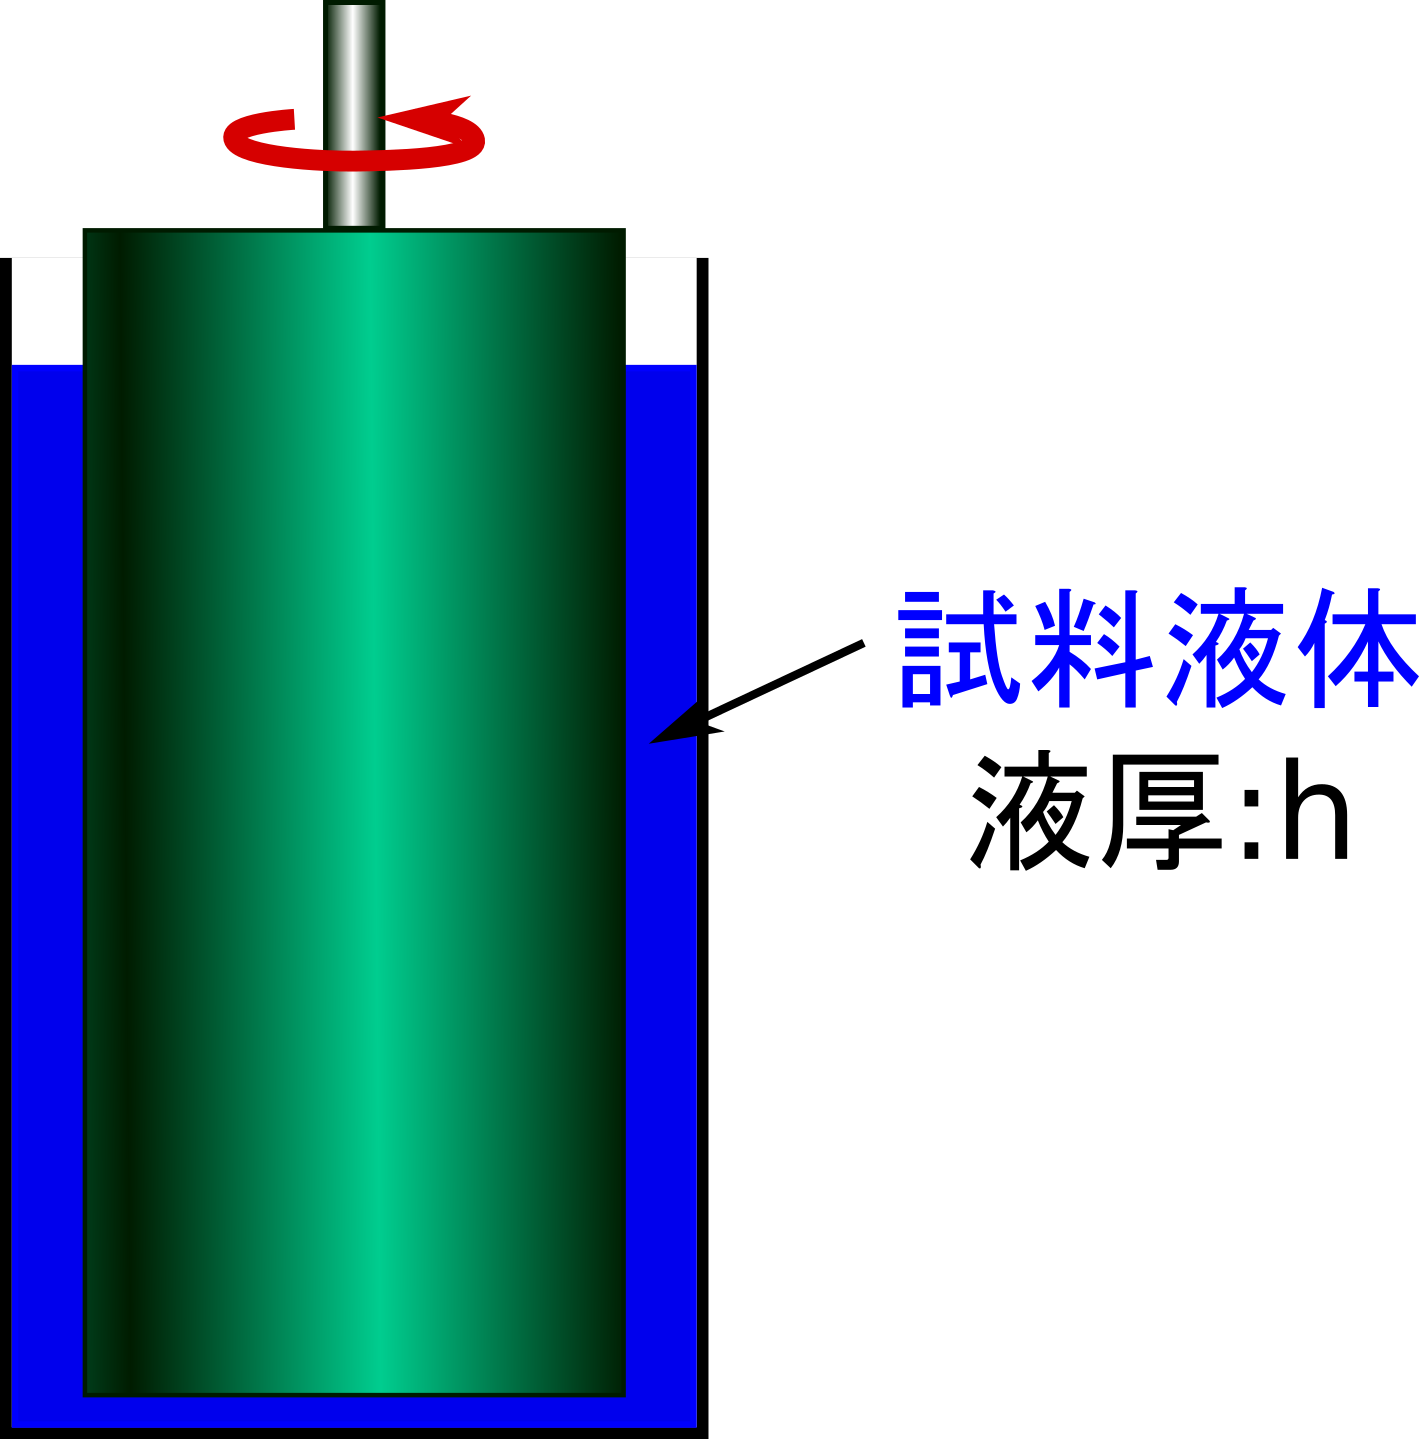
\includegraphics[width=.8\textwidth]{nijyu_entou.png}
			\end{center}
		\end{minipage}
		\caption{二重円筒による測定}
		\label{nijyu}
	\end{center}
\end{figure}

なお、粘度\index{ねんど@粘度}の単位は以下のようになります。
\begin{align}
	[\text{粘度}] &= \dfrac{[\text{せん断応力}]}{[\text{せん断速度}]} \notag \\
		&= \dfrac{[\mathrm{Pa}]}{[\mathrm{s^{-1}}]} = [\mathrm{Pa\cdot s}]
\end{align}


\subsubsection{液体\index{えきたい@液体}の力学モデル}

ニュートンの法則が成り立つような液体\index{えきたい@液体}の力学モデルをイメージ図とすると、図 \ref{flow_model} となります。
\begin{figure}[htbp]
	\begin{center}
		\begin{minipage}{0.55\textwidth}
			\large
			\begin{itembox}[l]{液体のモデル}
				\begin{itemize}
					\item 液体の振る舞いを表すモデル
					\item 右図のダッシュポット
					\item イメージとしては、水鉄砲
					\item 速くピストンを動かすと、\\抵抗が大。
				\end{itemize}
			\end{itembox}
			
		\end{minipage}
		\begin{minipage}{0.35\textwidth}
			\begin{center}
			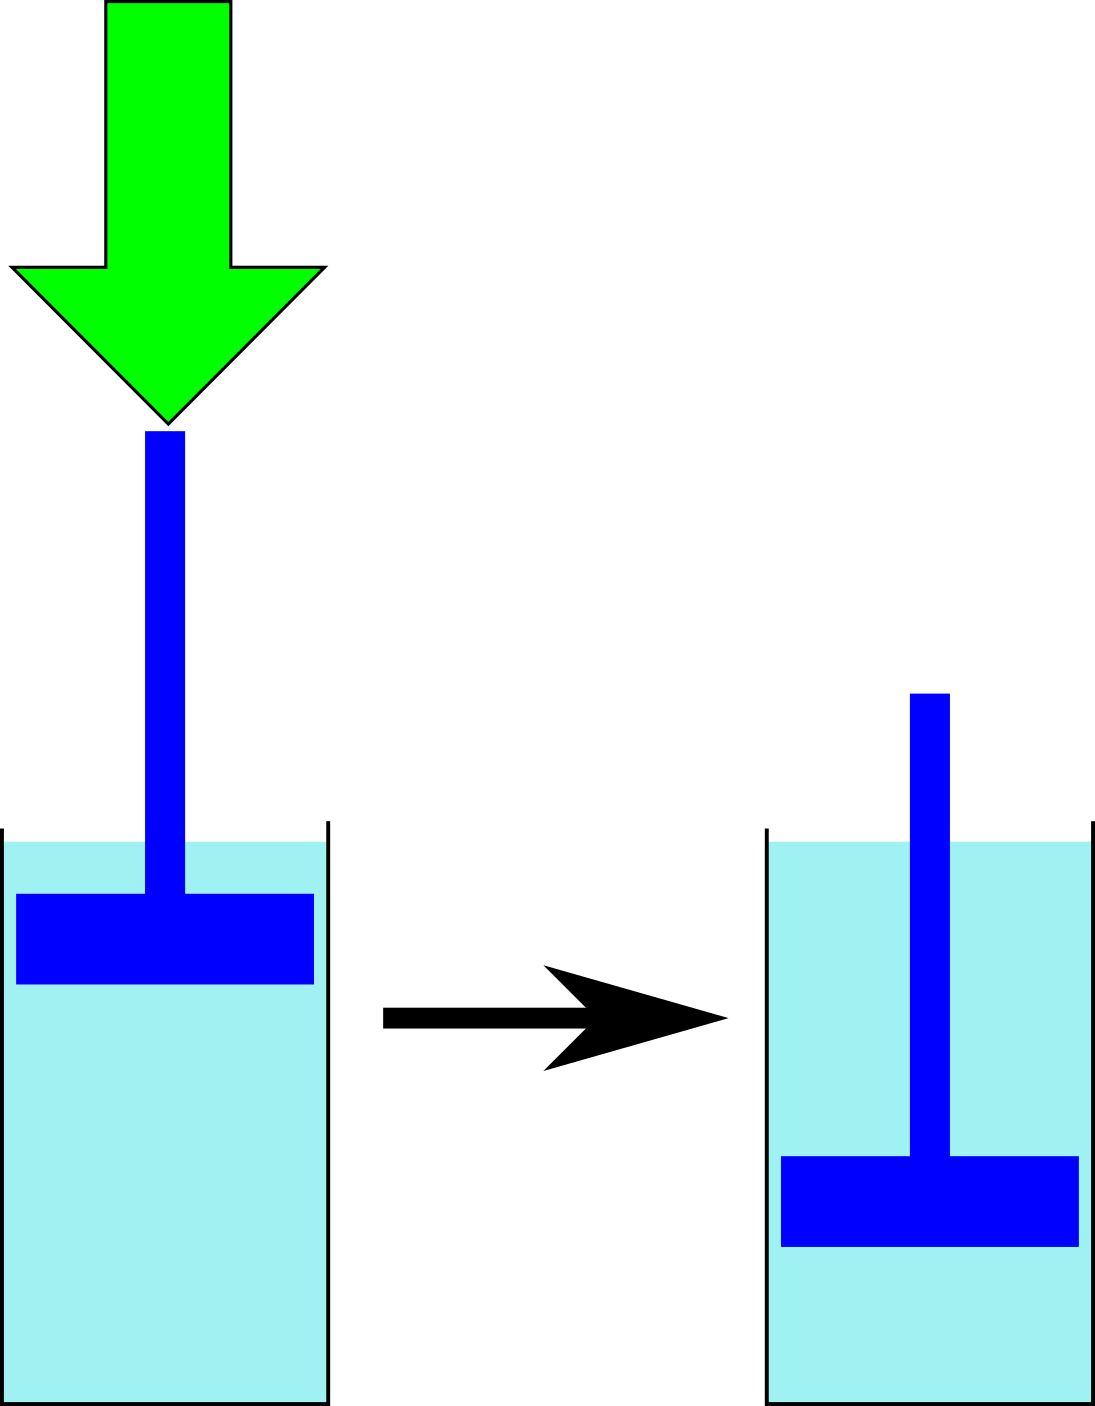
\includegraphics[width=.8\textwidth]{dashpot.png}
			\end{center}
		\end{minipage}
		\caption{液体の力学モデル}
		\label{flow_model}
	\end{center}
\end{figure}

このモデルは、液体\index{えきたい@液体}の抵抗がその変形速度に比例するというニュートン流体の特性を表しています。

\section*{この章のまとめ}

この章では、固体と液体という基本的な物質のふるまいを書き表す一番単純なモデルについて、説明を進めました。
	\begin{boxnote}
		\large
		\begin{itemize}
			\item 固体と液体という基本的な物質のありようについて、レオロジー的に考えていきます。
			\begin{itemize}
				\item 固体の最も基本的なモデルである弾性体という状態
				\item 刺激と応答を表すために、ひずみと応力を使うことで力学モデルが書けること
				\item 液体の応答について
				\item 液体の力学モデルが、「ひずみ速度\index{ひずみそくど@ひずみ速度}」で表されること
			\end{itemize} 
		\end{itemize}
	\end{boxnote}

	\newpage

	\begin{longartdeco}
		\begin{center}
		\emph{コラム:カエルの話}	
		\end{center}
	
		早逝されてしまった、元レオロジー学会長の上田さんという方がレオロジーの学び方のポイントとして、カエルの話をしていました。せっかくなので残して行きたいなと思い、ここに書いておくことにします。

	最初の話は、「茹でガエル」というもので、環境変化に関する寓話です。
	これは、1960年代の東西冷戦、1980年代の終末論、1990年代には温暖化に関連して取り上げられてきているようです。

	2つ目の話は、イソップ寓話に収録されている「二匹のカエル」というお話で、困難な状況でも頑張れば道は開ける(かも)というものです。
	上田さんは強引にクリームのダイラタンシーの話にしてレオロジーとつなげていました。
	結局、どっちのやり方がいいのかは、結果を見るまではわからないということなんで、自分のやり方を信じるしかないですね。

	「茹でガエル」

	カエルのような変温動物は、外部の温度環境によって自身の温度が変化します。
	したがって、本来は、気温が高くなって暑い場合は冷たい場所へ、また、気温が下がって凍えるときには暖かい場所へと移動する必要があります。
	カエルを熱い湯の中に入れてみると、居心地の良い場所へと慌てて逃げ出して行きます。
	でも、カエルを水の入ったビーカーに入れてゆっくりと水の温度を上げていくと、カエルは周りの温度が上がったことに気づかなくて、そのまま茹で上がって死んでしまいます。
	と書きましたが、これは似非科学的な作り話とのことです。

	人間も周りの環境が徐々に変化していっても気づかなくて、「アッと気づいたとき」には、逃げようのないとんでもない状況に追い込まれることがあります。
	ここから転じて、以下のような警句を表しています。
	「現状認識をしっかりと!」
	これは、周囲の変化に対して、常にきちんと対応しましょうということですね。

	「二匹のカエル」

	二匹のカエルが、ミルクのいっぱい入った壺の縁の周りを飛び跳ねていましたが、突然、二匹とも壺に落ちてしまいました。
	一匹のカエルは、「ああ、もう駄目だー!」と諦めてしまって、じっとして、結局溺れて死んでしまいました。
	もう一日のカエルは、「なんとかしよう」ともがいて、何度も何度も足を蹴って一生懸命泳ぎました。すると、足元のミルクがだんだんとチーズになって固まってきて、それを足がかりにして壺の外へと飛び出せました。
	これから得られる警句は、
	「現状分析するよりも行動を!」
	ということになります。
	まあ、変に周りが見えると、小賢しい考えにとらわれるので良くない場合もあるということです。
	
	\end{longartdeco}

\end{document}